\documentclass{standalone}

\usepackage{tikz}
\usetikzlibrary{shapes,arrows}

\tikzstyle{block} = [rectangle, draw, text centered, rounded corners, minimum
height=4cm, minimum width=2cm]

\tikzstyle{Mblock} = [rectangle, draw, text centered, rounded corners, minimum
height=0.5cm, minimum width=0.25cm]

\tikzstyle{blank} = [node distance = 0.8cm]
\tikzstyle{connectPoint} = [node distance = 1cm,circle,fill=black, inner sep= 0.5pt]

\tikzstyle{line} = [draw,->]
\tikzstyle{lineC} = [draw]

\tikzstyle{phaseShifter} = [circle,draw]


\begin{document}
 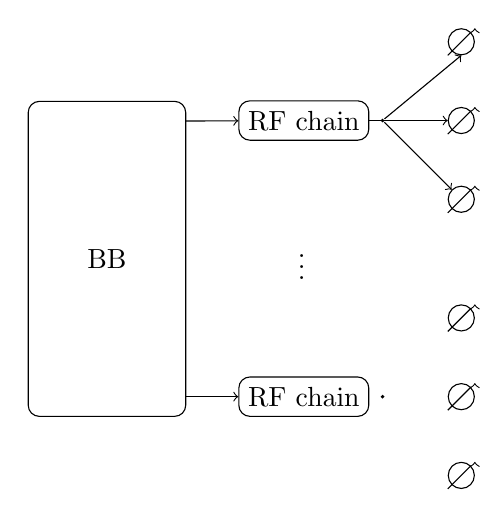
\begin{tikzpicture}

   \node[block] (dBeam) {BB};

   \node[Mblock] (RF1) [right of = dBeam, right = 1.5cm, above = 1.5cm] {RF chain};
   \node[Mblock] (RF2) [below of = RF1,below = 2.25cm] {RF chain};

   \node[blank]  (p1)  at (dBeam.east)[yshift=1.75 cm,xshift=-0.13cm] {};
   \node[blank]  (p2)  at (dBeam.east)[yshift=-1.75 cm,xshift=-0.13cm] {};

   \node[blank]  (dots) [right of = dBeam, right = 1.5cm] {$\vdots$};

   \node[connectPoint]  (nodeInOut1) [right of = RF1] {};
   \node[connectPoint]  (nodeInOut2) [right of = RF2] {};


   % Phase shifters of RF chains One
   \node[phaseShifter] (P1) [right of = nodeInOut1] {} ;
   \node[phaseShifter] (P2) [above of = P1] {} ;
   \node[phaseShifter] (P3) [below of = P1] {} ;


      % Phase shifters of RF chains One
   \node[phaseShifter] (W1) [right of = nodeInOut2] {} ;
   \node[phaseShifter] (W2) [above of = W1] {} ;
   \node[phaseShifter] (W3) [below of = W1] {} ;

   %% Lines

   \path[line] (p1) -- (RF1);
   \path[line] (p2) -- (RF2);
   \path[line] (RF1) -- (P1);
   \path[line] (nodeInOut1) -- (P2.south);
   \path[line] (nodeInOut1) -- (P3.north west);



   % Arrows of RF one
   \draw[->]   (P1.south west)+(-0.05,-0.05) -- (P1.north east)+(0.05,0.05);
   \draw[->]   (P2.south west)+(-0.05,-0.05) -- (P2.north east)+(0.05,0.05);
   \draw[->]   (P3.south west)+(-0.05,-0.05) -- (P3.north east)+(0.05,0.05);

      % Arrows of RF one
   \draw[->]   (W1.south west)+(-0.05,-0.05) -- (W1.north east)+(0.05,0.05);
   \draw[->]   (W2.south west)+(-0.05,-0.05) -- (W2.north east)+(0.05,0.05);
   \draw[->]   (W3.south west)+(-0.05,-0.05) -- (W3.north east)+(0.05,0.05);
   
  
\end{tikzpicture}
\end{document}


%%% Local Variables:
%%% mode: latex
%%% TeX-master: t
%%% End:
